\chapter{7 TeV and 8 TeV Differential Cross Section Measurement: Fitting and Unfolding}
\label{c:Differential_Cross_Section:fitting_and_unfolding}

\section{Maximum Likelihood Fit}
\label{maximum_likelihood_fit}
A simultaneous fit is done with three templates in bins of each variable.
- V\_Jets template combined over all global variable bins.
- QCD template also inclusive over all global variable bins

\subsection{Choice of templates}
\label{choice_of_templates}

\subsection{7TeV V+Jets Template}
\label{ss:7TeV_vplusjets_template}
Explain scaling of 8\TeV W and Z+Jets systematics sample templates to 7\TeV central normalisation.
    Using 8 TeV VJets systematic samples for 7 TeV so need to scale:
    vjets ratio = sigma(7TeV)*lumi(7TeV)/(sigma(8TeV)*lumi(8TeV))
    vjets\_ratio = ( 31314 * 5050 ) / ( 36257.2 * 19584 )

\subsecton{Fit Results}
\label{ss:fit_results}
- Plots
- Tables in appendix

\section{Unfolding}
\label{ss:unfolding}
		- SVD Unfolding
		- Pull distributions

\subsection{Measurement}
\label{ss:measurement}
TODO: THIS SECTION TAKEN STRAIGHT FROM AN AT THE MOMENT, NEED TO REWRITE.
%TODO: THIS SECTION TAKEN STRAIGHT FROM AN AT THE MOMENT, NEED TO REWRITE.

Once the number of \ttbar events ($\Nttbar$) is unfolded (see section \ref{ss:unfolding}) the normalised
differential cross-section is calculated for every bin $i$ of the measured variable. Firstly the cross-section in each bin is
defined as
\begin{equation}\label{eq:finll_1}
\Delta\sigttbar^i = \frac{\Nttbar^i}{\mathrm{BR} \times \epsilon \times {\cal L}} 
\end{equation}
where BR is the branching ratio of the semi-leptonic decay channel calculated using MC, $\epsilon$ the \ttbar efficiency
and ${\cal L}$ the measured luminosity. Since the efficiency is corrected for in the unfolding it is set to $1$.
Next the average value for the cross-section in each bin is obtained by dividing by the bin width $\Delta \mathrm{X}$:
\begin{equation}
\frac{\mathrm{d}\sigttbar^i}{\mathrm{d} \mathrm{X}} =
\frac{\Delta\sigttbar^i}{\Delta \mathrm{X} } = \frac{\Nttbar^i}{\mathrm{BR} \times {\cal L} \times \Delta \mathrm{X}} 
\end{equation}
Finally the average cross-section in each bin is normalised to the total measured cross-section
\begin{equation}
\label{eq:normalisedxs}
\frac{1}{\sigttbar^\mathrm{tot}} \frac{\mathrm{d}\sigttbar^i}{\mathrm{d} \mathrm{X}} =
\frac{1}{\sum\limits_{j}{\mathrm{d}\sigttbar^j}} \frac{\mathrm{d}\sigttbar^j}{\mathrm{d} \mathrm{X}} =
\frac{\mathrm{BR} \times {\cal L}}{\sum\limits_{j}{\Nttbar^j}}\frac{\Nttbar^i}{\mathrm{BR} \times {\cal L} \times \Delta
\mathrm{X}} = \frac{1}{\sum\limits_{j}{\Nttbar^j}}\frac{\Nttbar^i}{\Delta\mathrm{X}}
\end{equation}
This normalised cross-section distribution is not normalised to 1 as $\sigttbar^\mathrm{tot}$ does not take the bins
into account. However, if one was to include the bin widths in the normalisation then the information about the
bin-width would be lost in the measurement.

\subsection{Treatment of Systematic Uncertainties}
\label{ss:treatment_of_systematic_uncertainties}
		- How we deal with systematics
		- tables
		
Tau energy: The met energy systematics are electron energy up/down, muon energy up/down and tau energy
up/down. These systematics (and JES) are applied to both monte carlo and data. We found that the tau energy is
susprisingly high, considerably higher than the electron and muon energy systematics. We may select taus in
our signal region unintentionally although we don't select on taus. The signature of ttbar events with taus
can mimic the signature of electron + jets or muon + jets ttbar events. The image shows how taus decay. The W
from a top could decay to a tau, which would then decay either to a tau neutrino and a virtual W which then
decays to two jets which would be very close together (and therefore reconstructed as a single jet). Or, the
virtual W could decay to a lepton (electron or muon) and an associated neutrino). These signatures could fake
our signal, and therefore end up in our ttbar signal. In our unfolding, we remove fakes. However, we use the
shape of the fakes in the central to subtract from the signal distribution in the tau energy up/down
variations. The effect is not so pronounced in the electron up/down and muon up/down variations because there
are not many electrons or muons in the fakes. Luke found that \~14\% of the TTJet events we select on are NOT
from the decay we are looking for. This was by dividing the number of events in the fake ST distribution in
the unfolding histogram file by the number of events in the measured distribution (i.e. signal) in the same
file. The electron channel was actually ~13.5\% and the muon channel was actually ~13.9\%. The shape
comparison between the fakes and the signal shows that there are more fakes in the higher MET bins, which is
why the error in those bins is larger. These are likely to come from semi-leptonic tau events (where the tau
decays to a lepton and a neutrino); tau tau, e tau or mu tau where the tau decays hadronically; or ee, emu or mumu events where one of the leptons is lost (probably low fraction as well). So most of our fakes will include at least one tau. Since semi-leptonic tau would need to
decay leptonically, these taus are not identified and, I assume, not included in the MET uncertainty.

Looking at the shape difference between the central and tau up/down MET distributions, there is a significant
different (though not by much). Since this affects data, the difference goes through the fit, and the
unfolding, and is what we see in the final result. The difference in normalisation in the most affected bin is
\~6\%, suggesting that we have more than 6\% tau contamination overall (not sure if that is a correct
assumption). The normalisation across the bins does not change, of course, i.e. the sum of events in the bins
of, in this case MET, remain the same in the central measurement and in the tau energy up/down variations.
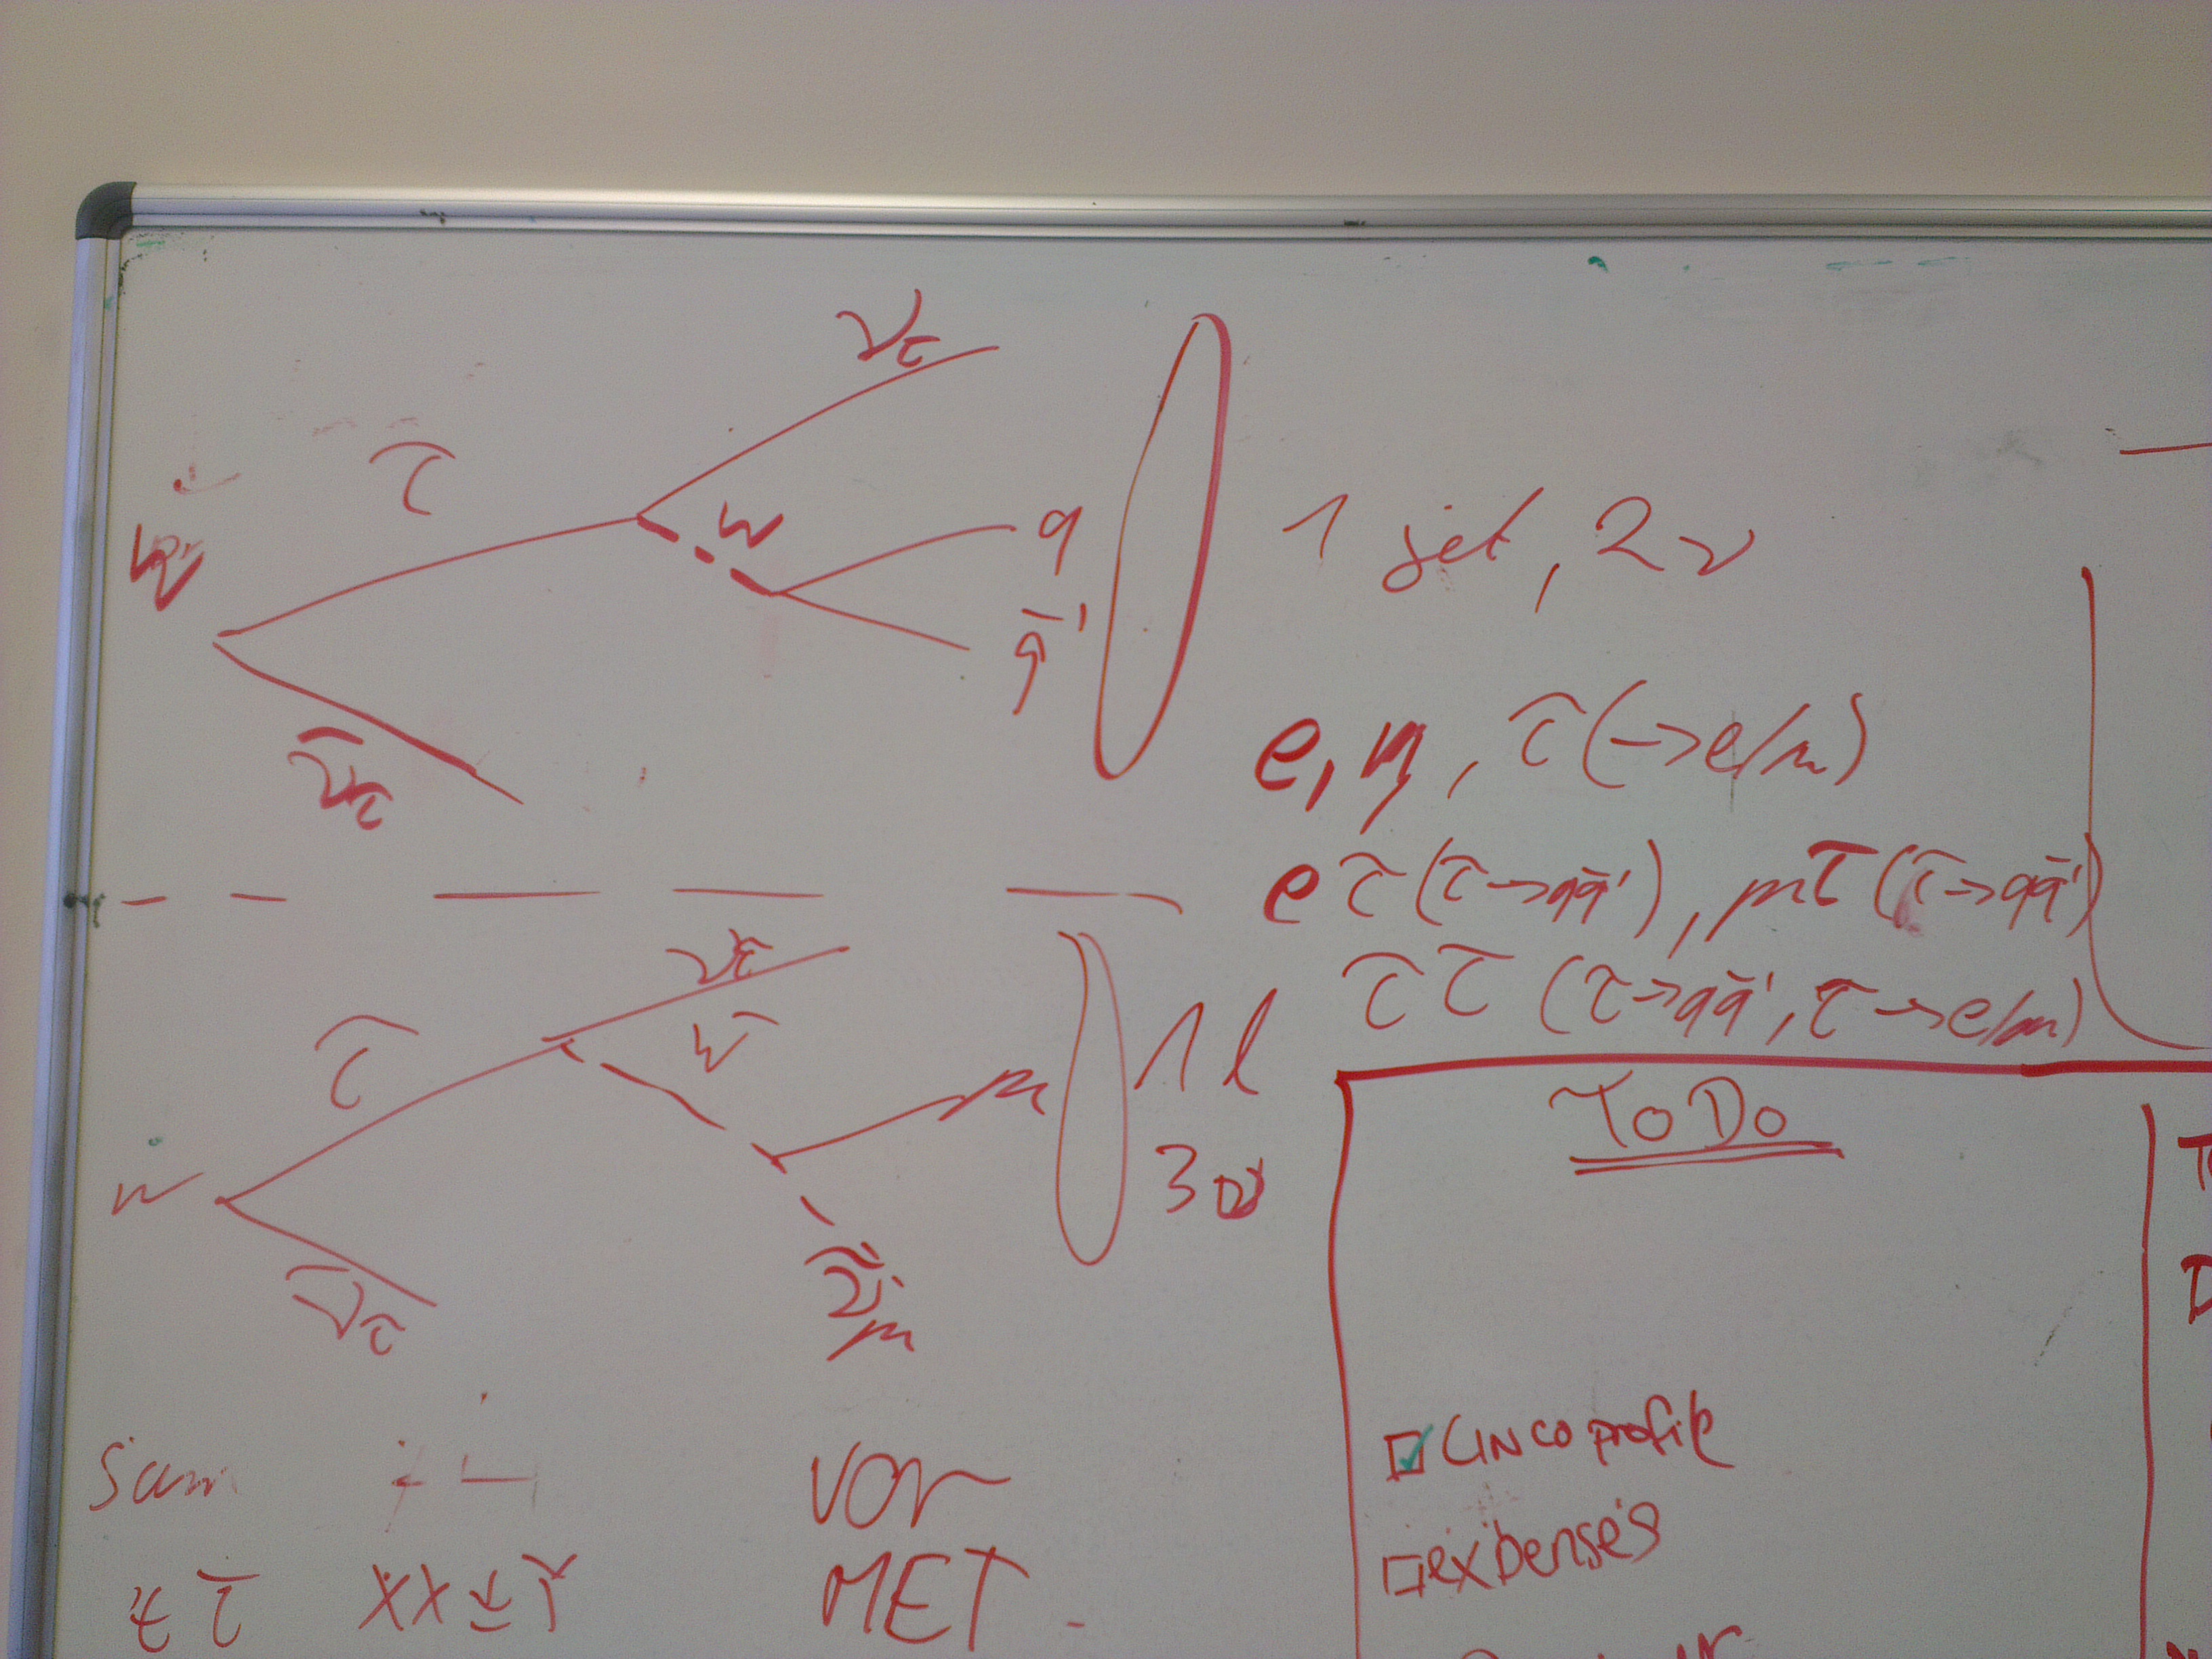
\includegraphics[width=\textwidth]{Chapters/04_Analysis/04b_XSections/Images/IMG_20150219_160840.jpg}
		